% Anexo · Acta de la reunión del 4 de septiembre (anexo obligatorio del enunciado).
% Se incrusta el PDF que se envió a la contraparte, sin modificar.
% Requiere pdfpages en el preámbulo.

\section*{Anexo. Acta de la reunión del 4 de septiembre}
\addcontentsline{toc}{section}{Anexo. Acta de la reunión del 4 de septiembre}

\noindent Enviada a la contraparte y al cuerpo docente el 8 de septiembre de 2026, dentro del plazo de 48 horas. Se reproduce sin modificaciones.

\medskip
\noindent\textbf{Nota de corrección (noviembre de 2026).} El acta afirma que la unidad de medida de la empresa es el litro. Es una lectura incorrecta de la reunión: operaciones mide en litros, mientras finanzas y comercial venden y hablan en cajas, y la contraparte reconoció no tener gobierno de datos sobre esa equivalencia (V). El texto enviado se conserva sin cambios; la corrección está en la sección~\ref{sec:mandato}.

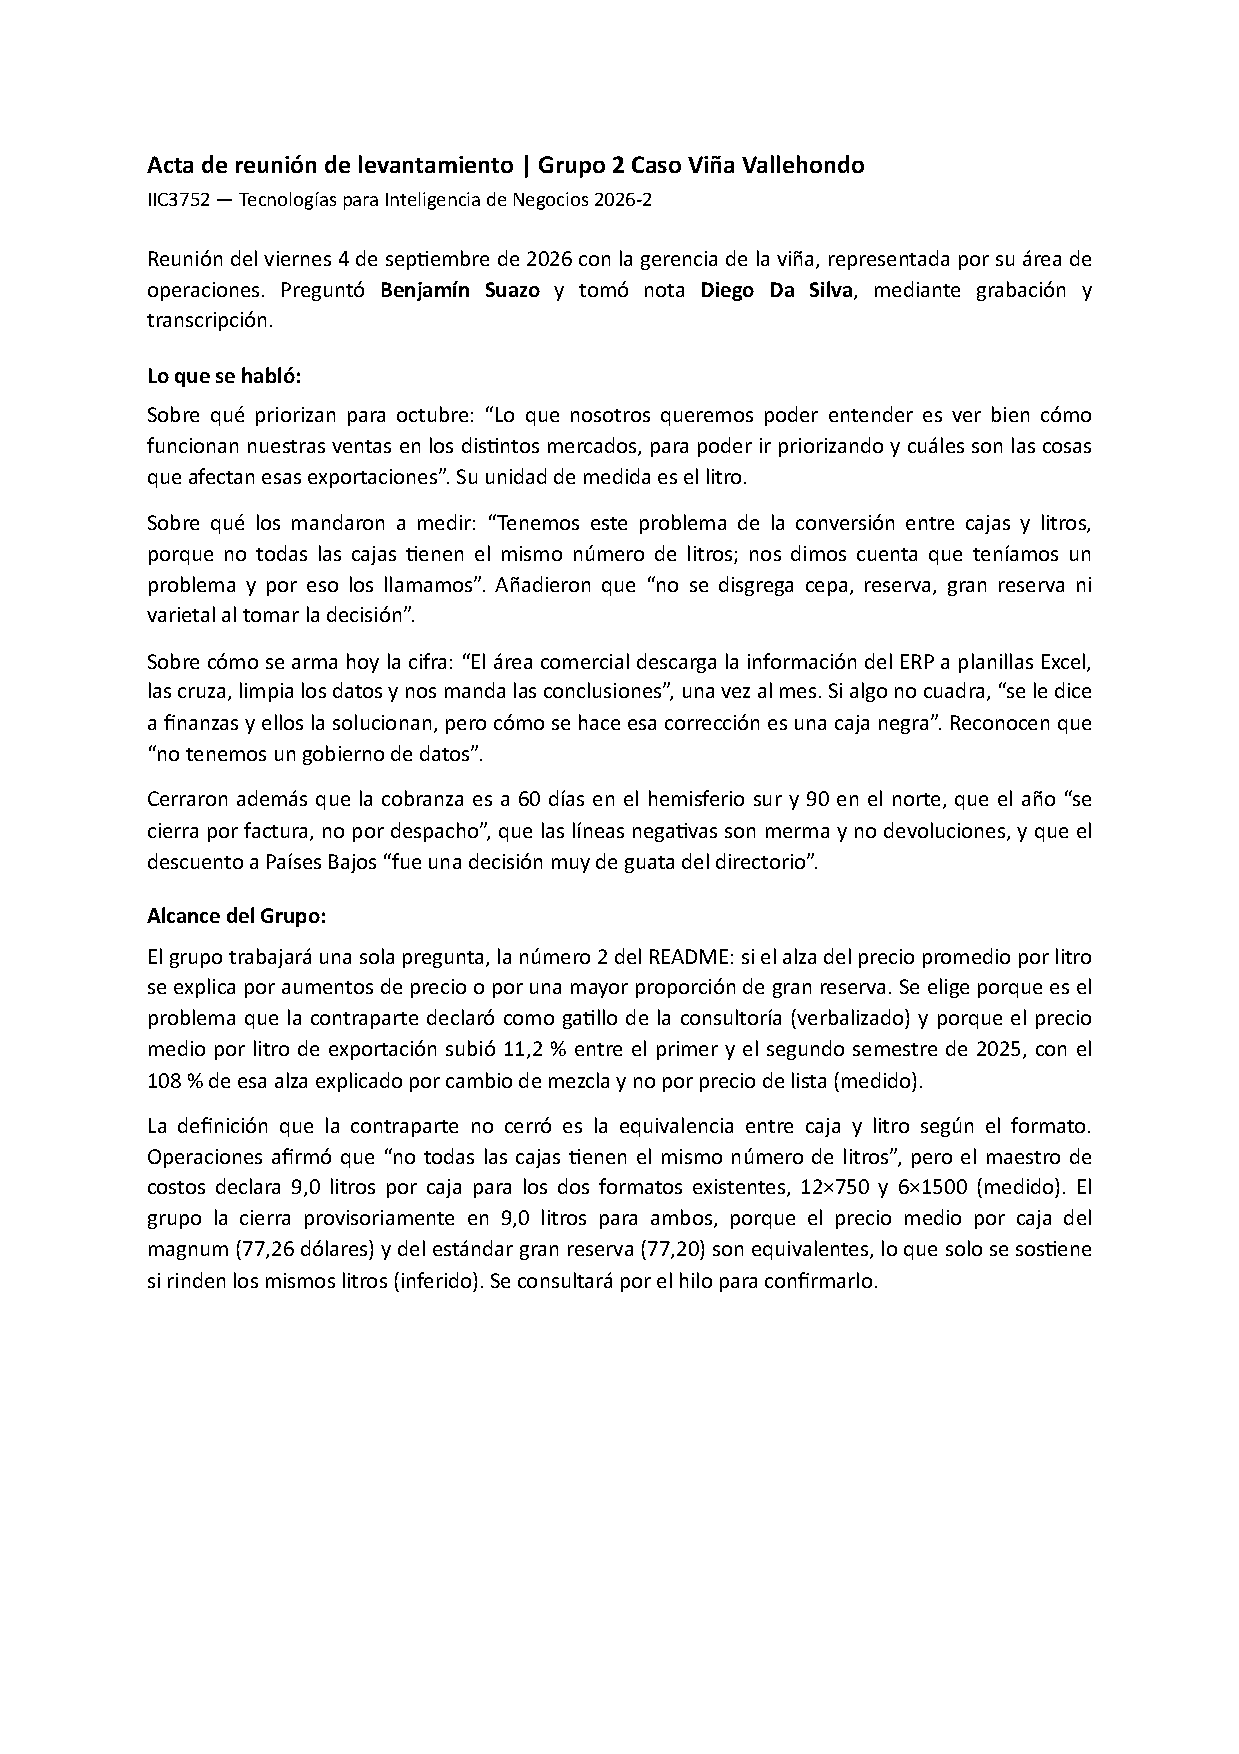
\includepdf[pages=-,scale=0.92]{anexos/Acta_Reunion_Vallehondo_G2.pdf}
